% Пример заготовки для презентации с использованием класса Beamer LaTeX.
% Версия от 09 ноября 2018 года.
\documentclass[12pt,a4paper,mathserif]{beamer}
\usepackage[english,russian]{babel}
% XeLaTeX по умолчанию не поддерживает CMR-шрифты, поэтому в данном шаблоне объявление шрифтов изменено
\usepackage{fontspec}
\setmainfont{CMU Serif}
\setsansfont{CMU Sans Serif}
\setmonofont{CMU Typewriter Text}
\usepackage{amsmath}
\usepackage{amsfonts}
\usepackage{amssymb}
\usepackage{mathtext}
\usepackage{graphicx}
\usepackage{enumerate}
\usepackage{multirow}
\usepackage{ragged2e}
% Пакет для оформления исходного кода
\usepackage{minted}
\usepackage{adjustbox}
% Пакет для удаления нумерации рисунков
\usepackage[labelformat=empty]{caption}
% Пакет для оформления исходного кода
\usepackage{minted}
\justifying
\renewcommand{\raggedright}{\leftskip=0pt \rightskip=0pt plus 0cm}
\setbeamertemplate{caption}[numbered]

\usetheme {Madrid}
\usecolortheme [RGB={47, 47, 107}]{structure}

\author[Лаптев А.В.]{{Cтудент 5.306М группы: Лаптев А.~В.}\\
{Научный руководитель: Калачев А.~В.}}
\title[Барнаул 2025]{\large Исследование и реализация методов автоматического распознавания CAPTCHA различных форматов на основе нейросетевых моделей}
% \subtitle{Отчет по научно-исследовательской работе}

\begin{document}
\begin{frame}
\maketitle
\end{frame}

\begin{frame}{Актуальность работы}
    \setlength{\parindent}{0.5cm}
    Актуальность данной работы обусловлена как возрастающей сложностью 
    CAPTCHA-систем, так и развитием инструментов, позволяющих преодолевать 
    защитные механизмы web-ресурсов.
    
    Анализ эффективности и разработка подходов для автоматизированного решению 
    CAPTCHA могут применяться не только с точки зрения изучения устойчивости 
    самих систем, но и в рамках исследования прикладного применения нейросетевых 
    моделей в задачах распознавания информации в условиях ограничений.
\end{frame}

\begin{frame}{Цель работы}
    \setlength{\parindent}{0.5cm}
    Целью работы является разработка и анализ комплексного подхода к 
    автоматизации решения CAPTCHA в различных форматах с использованием 
    современных нейросетевых инструментов и API для распознавания.
\end{frame}

\begin{frame}{Задачи работы}
    \setlength{\parindent}{0.5cm}
    Для достижения поставленной цели были сформулированы следующие задачи:

    \begin{enumerate}
        \item провести обзор существующих форматов CAPTCHA и методов их защиты;
        \item разработать систему автоматического распознавания текстовых CAPTCHA с 
        искажениями;
        \item реализовать подход к решению графических CAPTCHA на основе методов 
        компьютерного зрения и нейросетевых моделей;
        \item построить решение для аудио CAPTCHA с использованием средств 
        автоматического распознавания речи;
        \item протестировать реализованные решения в реальных условиях, оценить 
        точность распознавания и устойчивость к изменениям условий подачи данных.
    \end{enumerate}
\end{frame}

\begin{frame}{Популярные форматы CAPTCHA}
    \setlength{\parindent}{0.5cm}
    Проверочный код CAPTCHA -- метод защиты, основанный на принципе 
    аутентификации <<вызов-ответ>>, предназначен для предотвращения различных 
    автоматических действий путем выполнения пользователем простого теста, 
    подтверждающего, что он человек, а не программа.

    Наиболее популярными форматами CAPTCHA являются:

    \begin{enumerate}
        \item текстовый формат;
        \item аудио формат;
        \item графический формат.
    \end{enumerate}
\end{frame}

\begin{frame}{Пример CAPTCHA в текстовом формате}
    \begin{figure}
        \centering
        
\includegraphics[width=1\linewidth]{imgs/text-captcha.jpg}
    \end{figure}
\end{frame}

\begin{frame}{Пример CAPTCHA в аудио формате}
    \begin{figure}
        \centering
        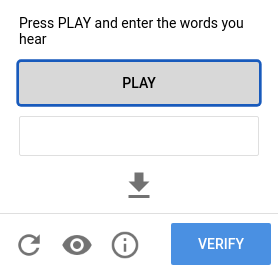
\includegraphics[width=0.55\linewidth]{imgs/audio-captcha.png}
    \end{figure}
\end{frame}

\begin{frame}{Пример CAPTCHA в графическом формате}
    \begin{figure}
        \centering
        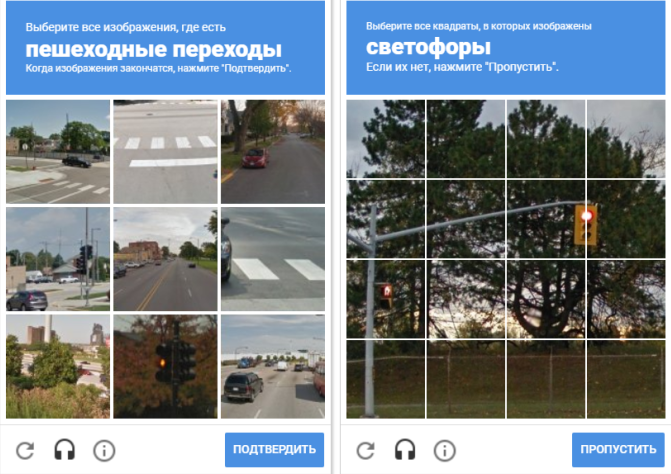
\includegraphics[width=0.85\linewidth]{imgs/image-captcha.png}
    \end{figure}
\end{frame}

\begin{frame}{\large Подходы к автоматизированному решению CAPTCHA}
    \setlength{\parindent}{0.5cm}
    Подходы, которые использовались для автоматизации решения CAPTCHA в различных 
    форматах:

    \begin{enumerate}
        \item аудио формат: облачный API с поддержкой продвинутых моделей 
        автоматического распознавания речи (ASR);
        \item текстовый формат: модель последовательного обучения \\(Seq2Seq) и 
        алгоритмы шумоподавления на изображениях;
        \item графический формат: одноэтапная модель для детекции объектов (YOLO) 
        с поддержкой сегментации.
    \end{enumerate}
\end{frame}

\begin{frame}{Обработка аудиофайла CAPTCHA}
    \setlength{\parindent}{0.5cm}
    Процесс обработки аудиофайла состоит из нескольких этапов:
    
    \begin{enumerate}
        \item преобразование формата аудиофайла;
        \item распознавание речи в аудиофайле;
        \item сохранение результата распознавания.
    \end{enumerate}

    \begin{figure}[H]
        \centering
        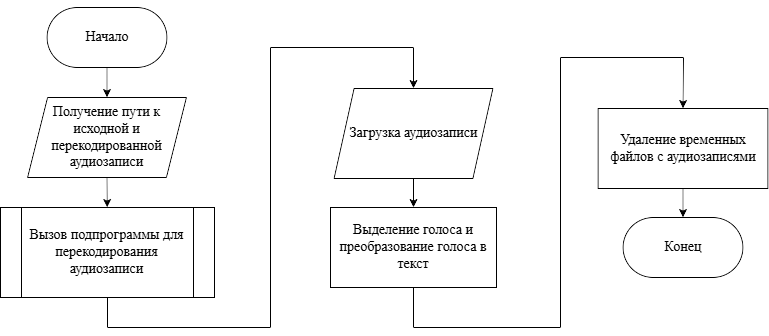
\includegraphics[width=0.8\linewidth]{imgs/flowchart-asr.png}
        \caption{Блок-схема процесса распознавания аудио CAPTCHA.}
    \end{figure}
\end{frame}

\begin{frame}{\small Тестирование решения для автоматизации решения аудио CAPTCHA}
    \begin{figure}
        \centering
        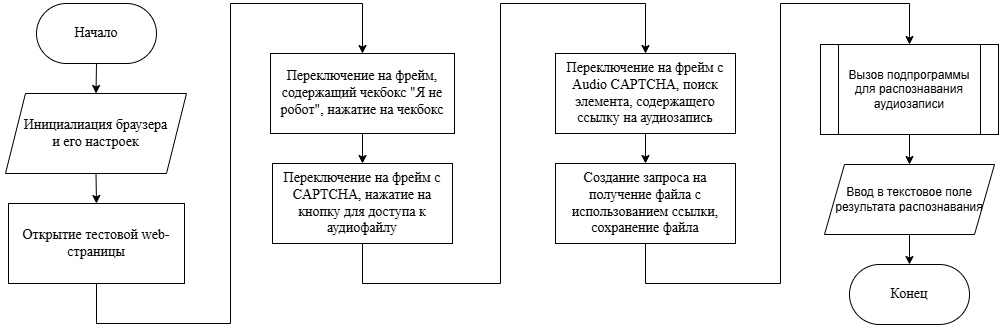
\includegraphics[width=1\linewidth]{imgs/flowchart-solve.png}
        \caption{Блок-схема процесса прохождения аудио CAPTCHA.}
    \end{figure}
\end{frame}

\begin{frame}{\large Подготовка датасета с текстовыми CAPTCHA}
    \setlength{\parindent}{0.5cm}
    Для обучения модели был создан датасет из 100 000 изображений с текстовыми 
    CAPTCHA, сгенерированными с использованием библиотеки captcha на Python. 
    Датасет включает в себя следующие символы: ABCDEFGHJKLMNPQRSTWXYZ23456789.

    Каждое изображение прошло этап предобработки, как показано на рисунке ниже:

    \begin{figure}[H]
        \centering
        \begin{minipage}[h]{0.45\linewidth}
            \center{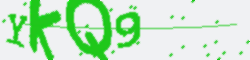
\includegraphics[width=1\linewidth]{imgs/YKQ9.png}} 
            \\ а)
        \end{minipage}
        \begin{minipage}[h]{0.45\linewidth}
            \center{
\includegraphics[width=1\linewidth]{imgs/YKQ9-preprocessing.png}} 
            \\ б)
        \end{minipage}
        \caption{\centering Изображения CAPTCHA: а) -- сгенерированное изображение, б) -- результат обработки.}
    \end{figure}
\end{frame}

\begin{frame}{\small Обучение модели для автоматизации решения текстовых CAPTCHA}
    \setlength{\parindent}{0.5cm}
    Исходный датасет был случайным образом перемешан и разделен на три 
    подмножества: обучающее, тестовое и валидационное в соотношении 80:10:10.

    \begin{figure}[H]
        \centering
        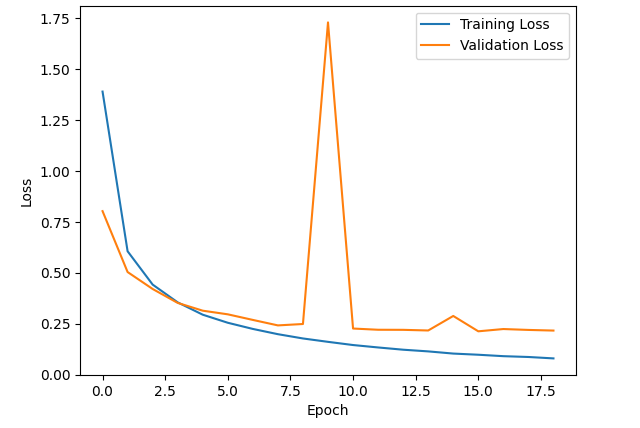
\includegraphics[width=0.57\linewidth]{imgs/model-loss.png}
        \caption{\centering График изменения значений функции потерь в процессе обучения модели для решения текстовых CAPTCHA.}
    \end{figure}
\end{frame}

\begin{frame}{\small Обучение модели для автоматизации решения текстовых CAPTCHA}
    \begin{figure}
        \centering
        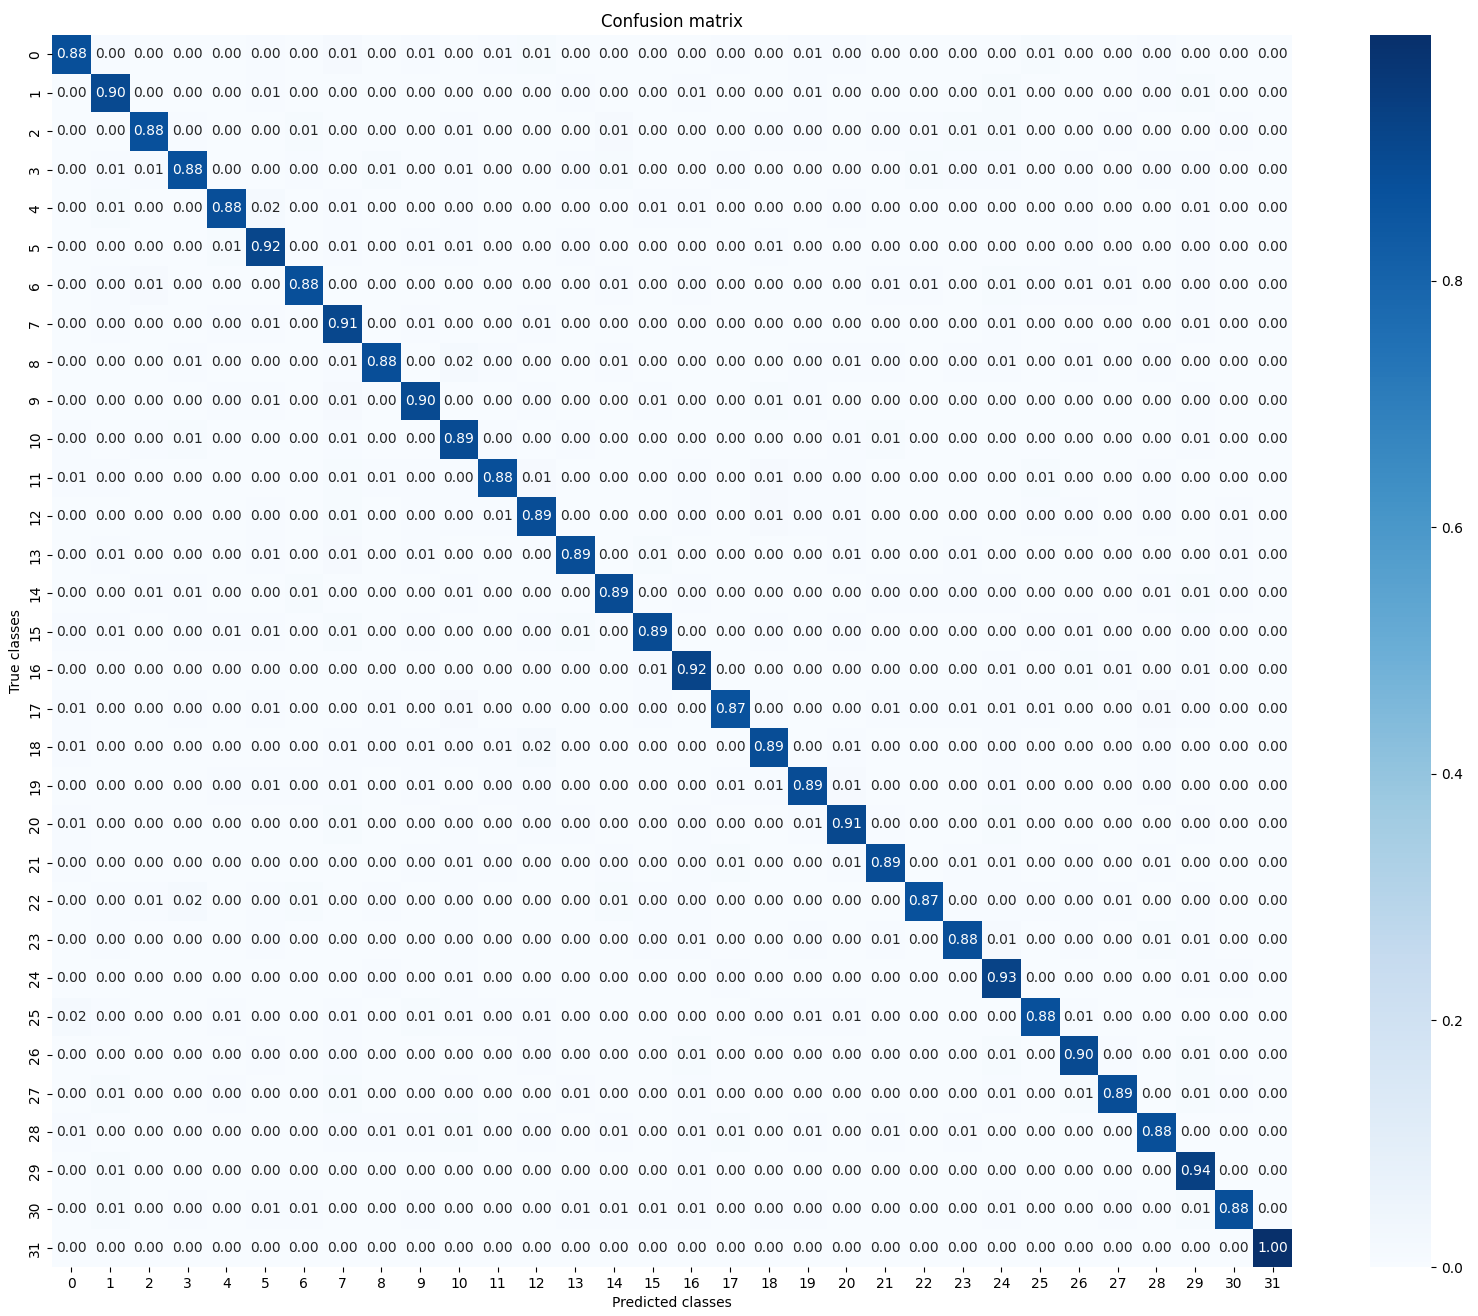
\includegraphics[width=0.63\linewidth]{imgs/confusion-matrix.png}
        \caption{\centering Матрица ошибок обученной модели для решения текстовых CAPTCHA.}
    \end{figure}
\end{frame}

\begin{frame}{\footnotesize Тестирование модели для автоматизации решения текстовых CAPTCHA}
    \setlength{\parindent}{0.5cm}
    Точность распознавания моделью отдельных символов составила 0.9263.

    Точность распознавания последовательностей различной длины представлена в 
    таблице ниже.

    \begin{table}[H]
        \centering
        \caption{Точность предсказаний для последовательностей различной длины.}
        \begin{tabular}{|l|l|}
            \hline
            Длина последовательности & Точность распознавания \\
            \hline
            4 символа & 0.9305 \\
            \hline
            5 символов & 0.7450 \\
            \hline
            6 символов & 0.4575 \\
            \hline
            7 символов & 0.1915 \\
            \hline
        \end{tabular}
    \end{table}
\end{frame}

\begin{frame}{\large Подготовка датасета с графическими CAPTCHA}
    \begin{figure}
        \centering
        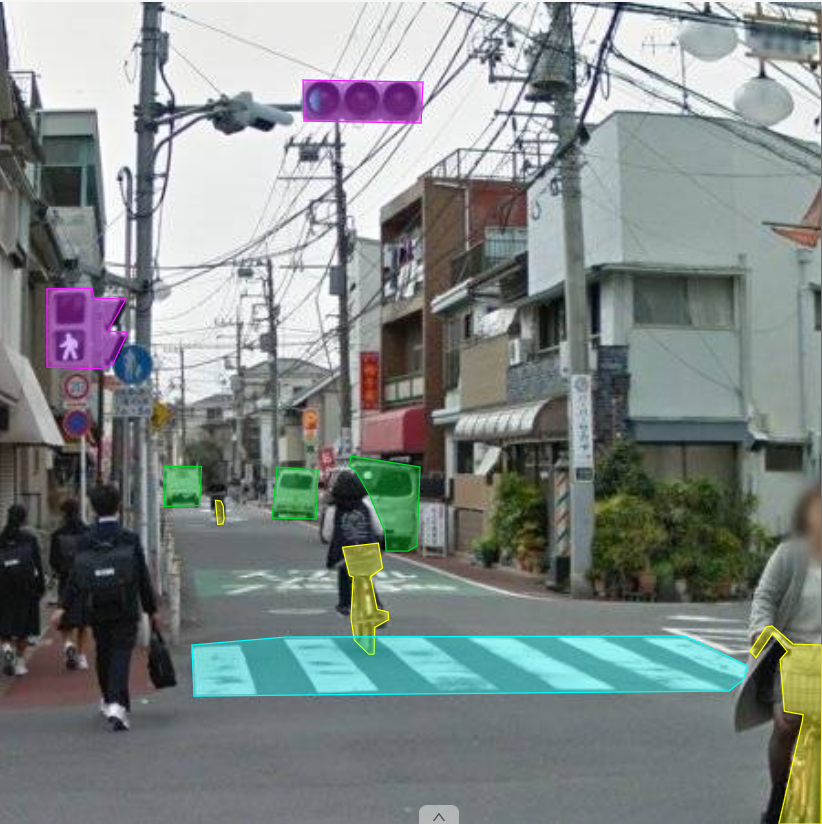
\includegraphics[width=0.55\linewidth]{imgs/captcha-poligons.png}
        \caption{Пример разметки изображения с тестовой графической CAPTCHA.}
    \end{figure}
\end{frame}

\begin{frame}[fragile]{\small Обучение модели для автоматизации решения графических CAPTCHA}
    \setlength{\parindent}{0.5cm}
    Набор классов, пути к выборкам и параметры конфигурации задаются в YAML-файле, 
    который передается при обучении модели. Содержимое такого файла для данной 
    модели:

    \inputminted[
        fontsize=\small,
        mathescape,
        linenos,
        frame=lines,
        breaklines
    ]{yaml}{code/train_captcha.yaml}
    \vspace{-0.5cm}
    \begin{center}
        Параметры конфигурации для обучения модели.
    \end{center}
\end{frame}

\begin{frame}{\small Обучение модели для автоматизации решения графических CAPTCHA}
    \begin{figure}
        \centering
        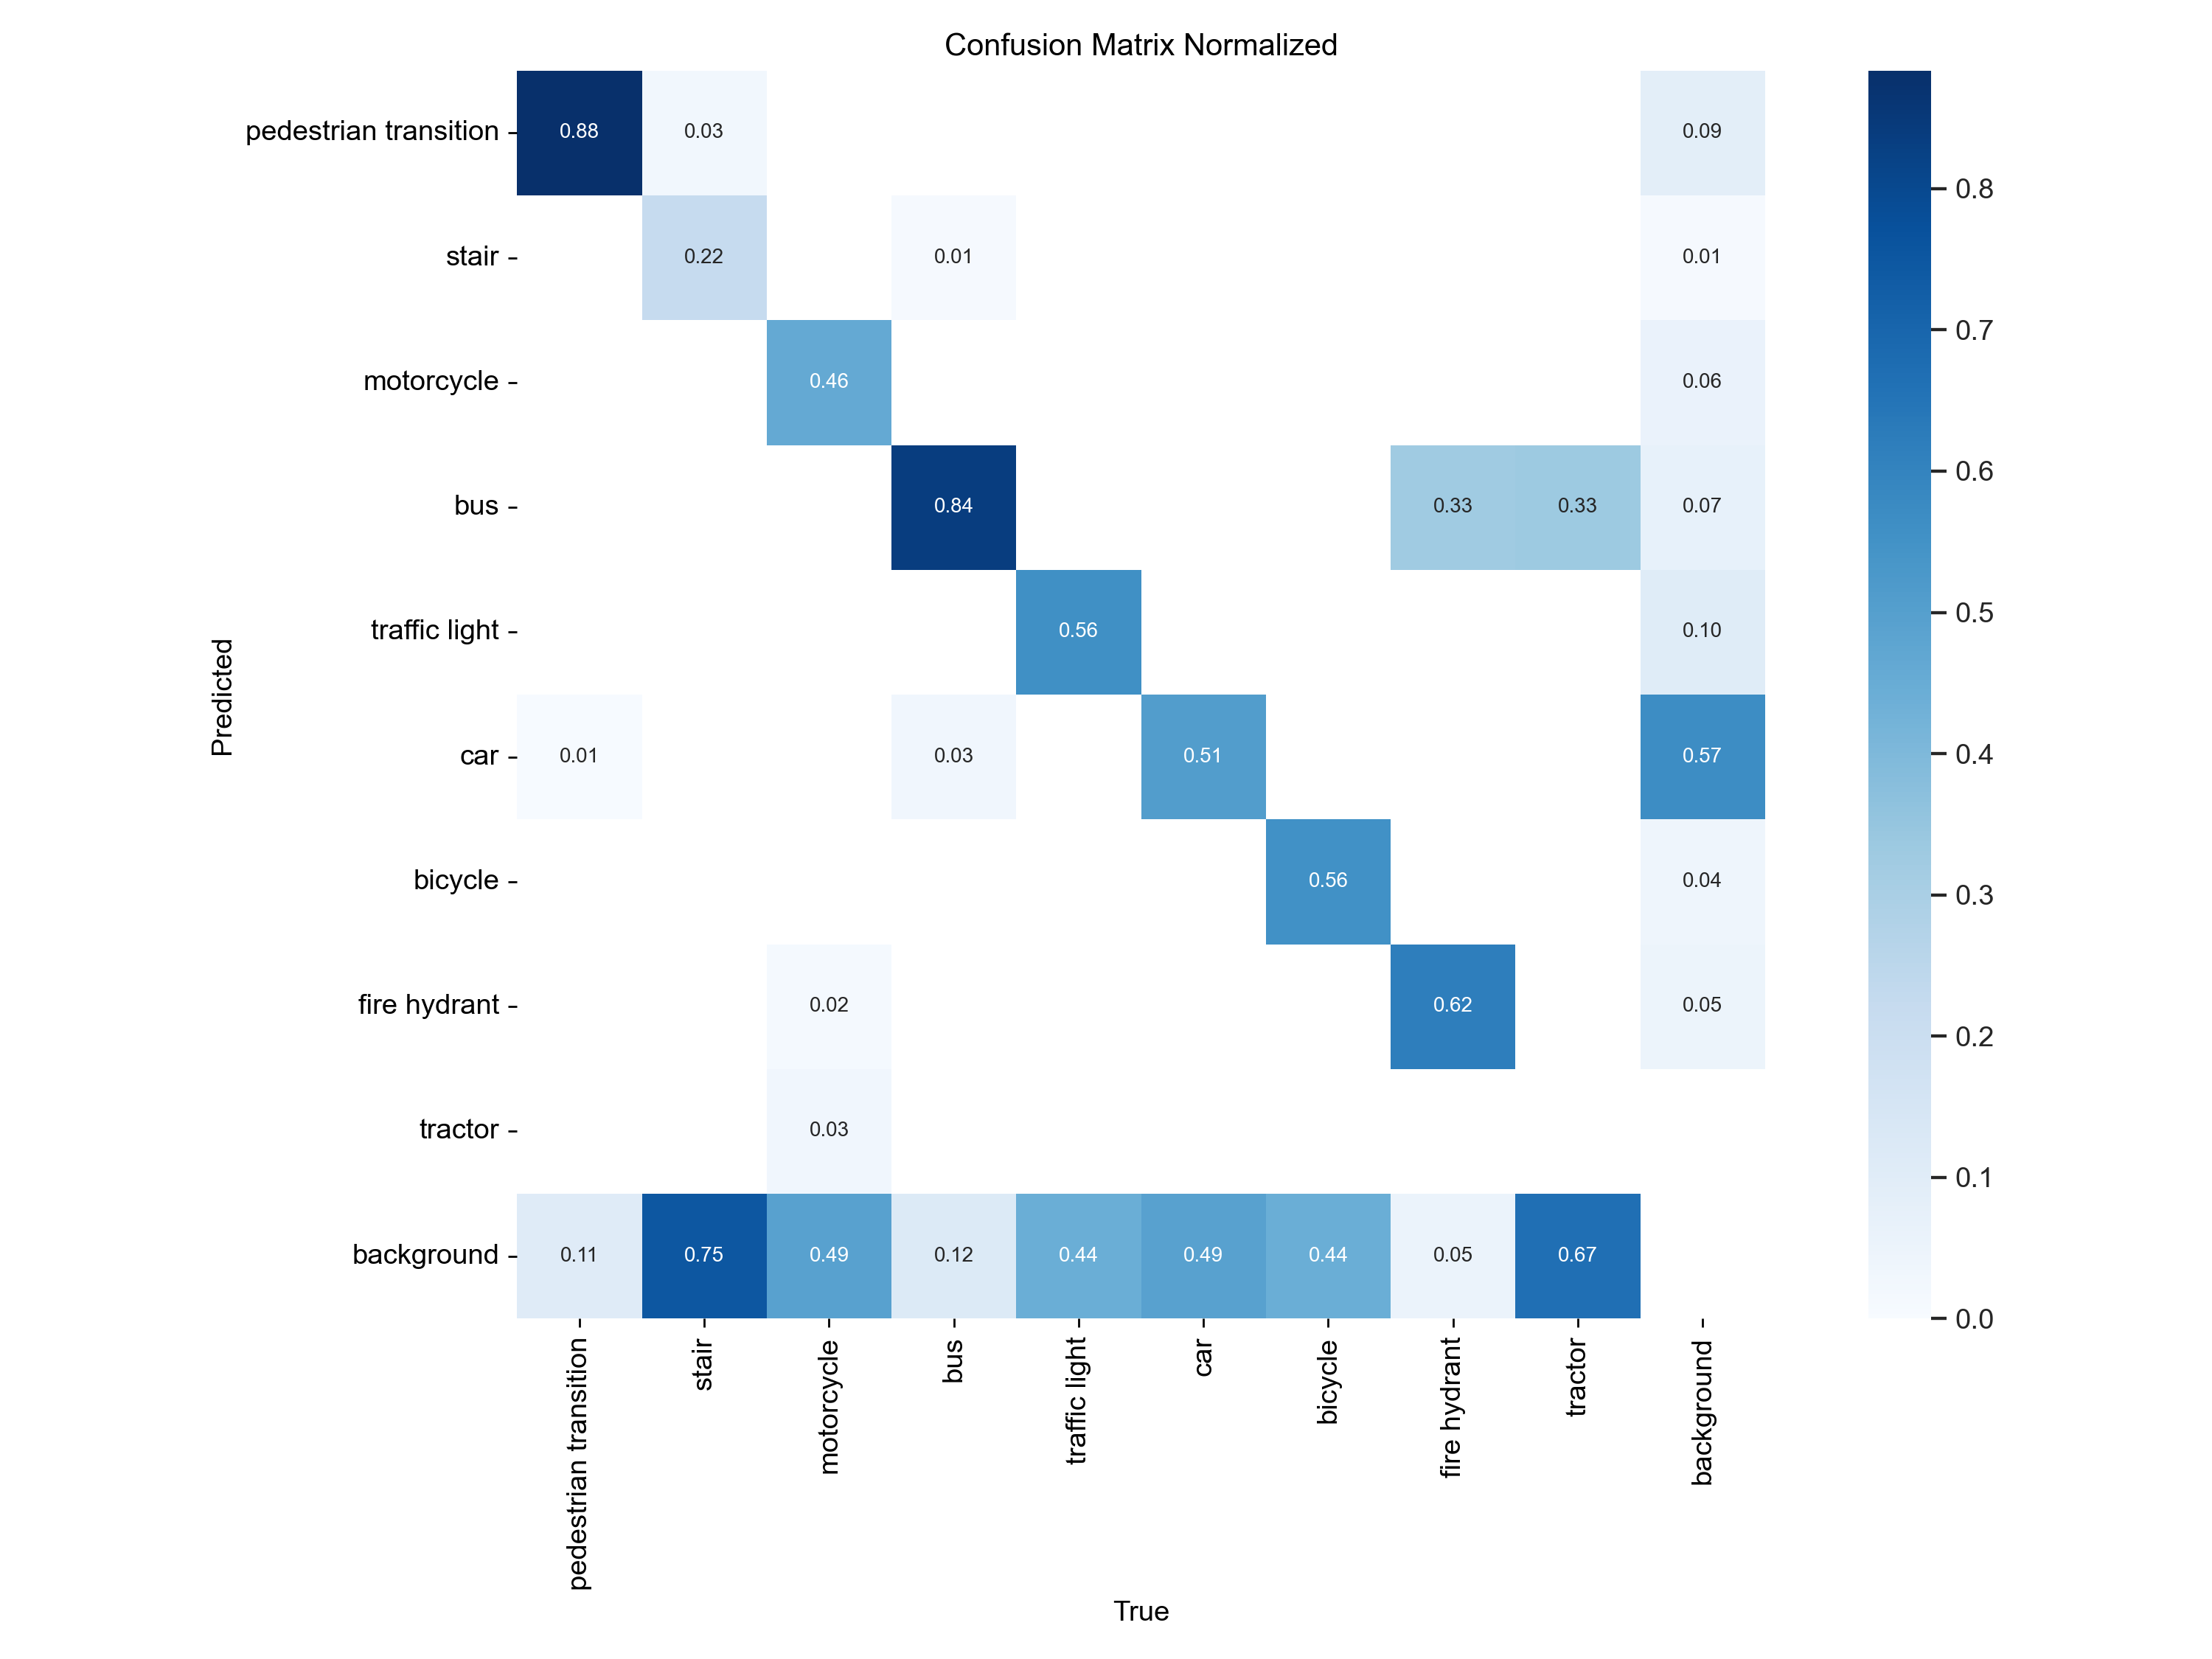
\includegraphics[width=0.68\linewidth]{imgs/confusion_matrix_normalized.png}
        \caption{\centering Матрица ошибок для изображений валидационной выборки для модели YOLOv8.}
    \end{figure}
\end{frame}

\begin{frame}{\small Обучение модели для автоматизации решения графических CAPTCHA}
    \setlength{\parindent}{0.5cm}
    Результаты обучения модели на основе YOLO отслеживались по ключевым метрикам 
    (IoU, Precision, Recall, Loss), которые визуализировались автоматически. 
    Примеры графиков с результатами обучения приведены ниже:

    \begin{figure}[H]
        \centering
        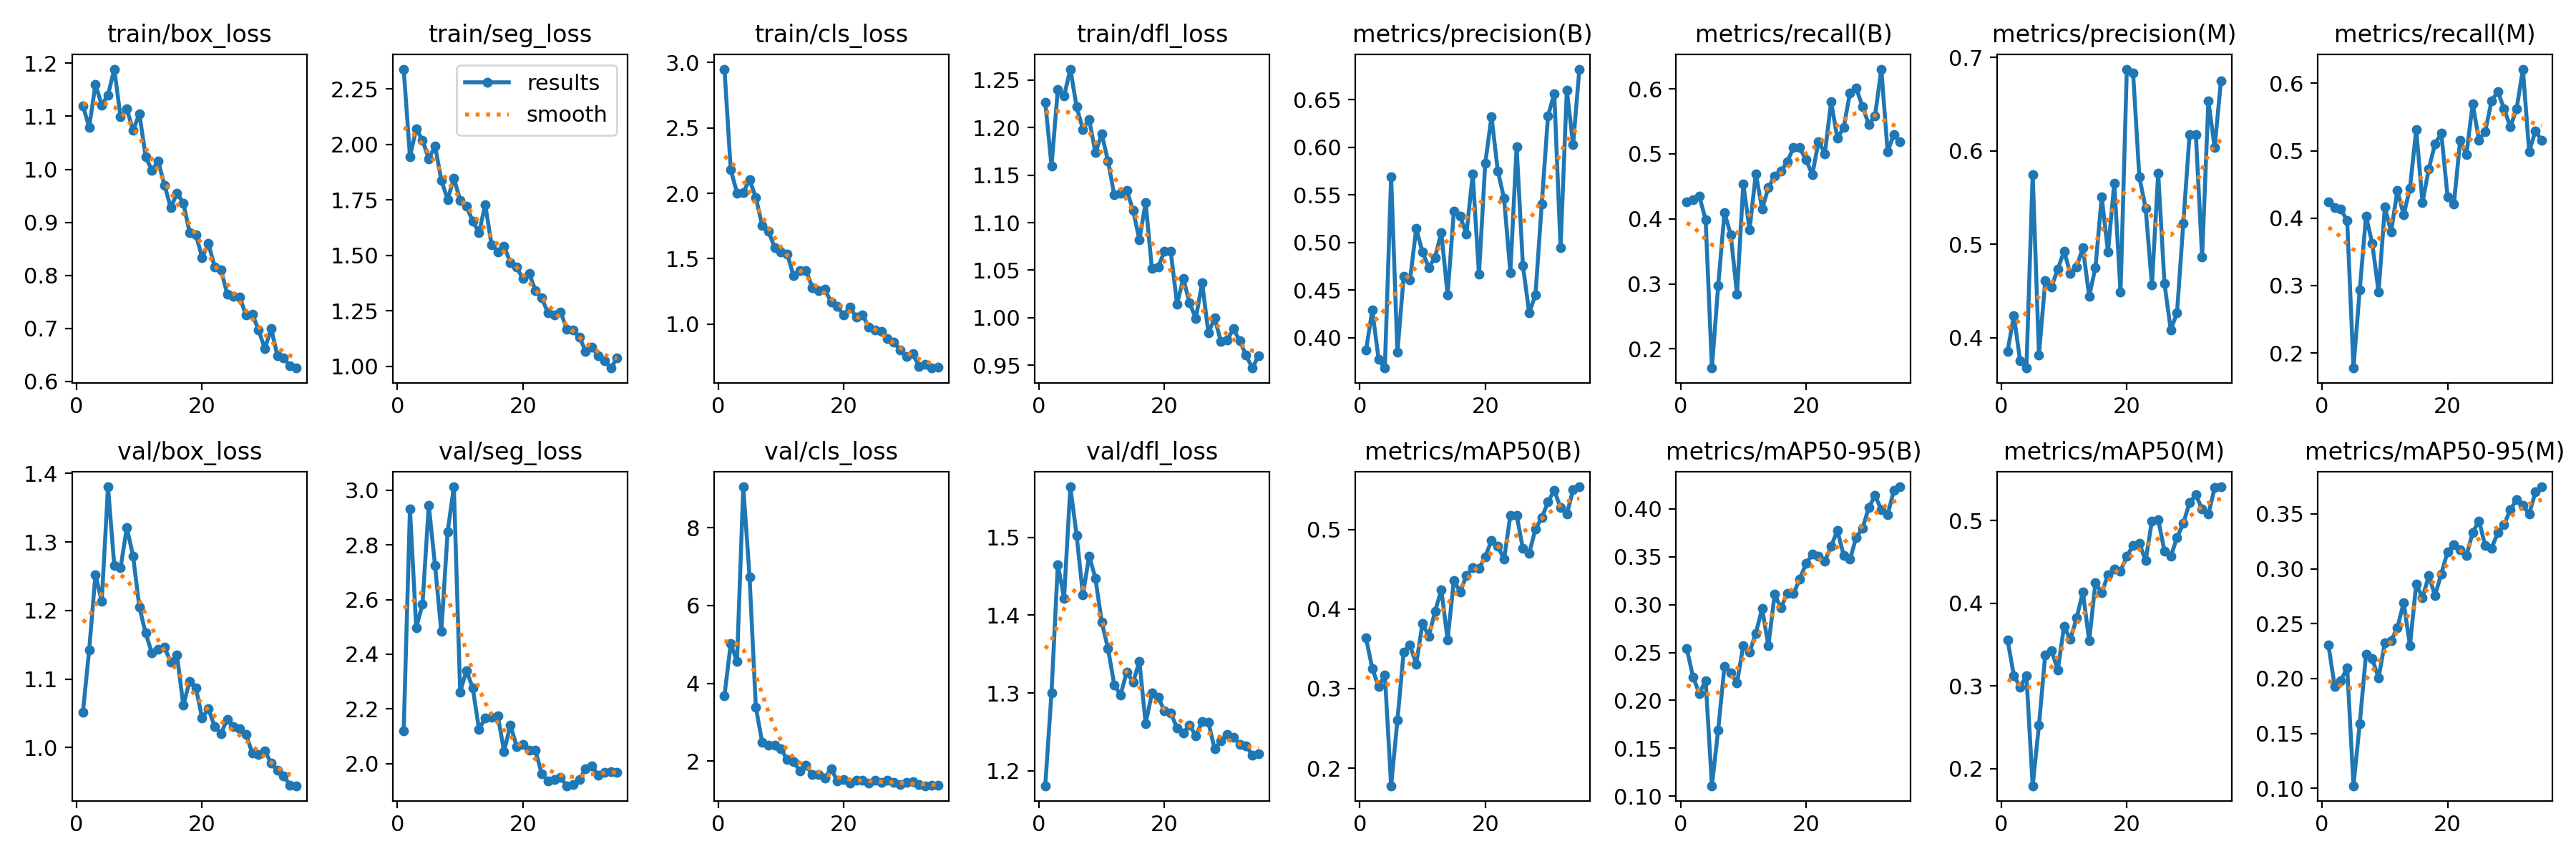
\includegraphics[width=1\linewidth]{imgs/results.png}
        \caption{Изменение ключевых метрик в процессе обучения модели YOLOv8.}
    \end{figure}
\end{frame}

\begin{frame}{\footnotesize Тестирование модели для автоматизации решения графических CAPTCHA}
    \begin{figure}
        \centering
        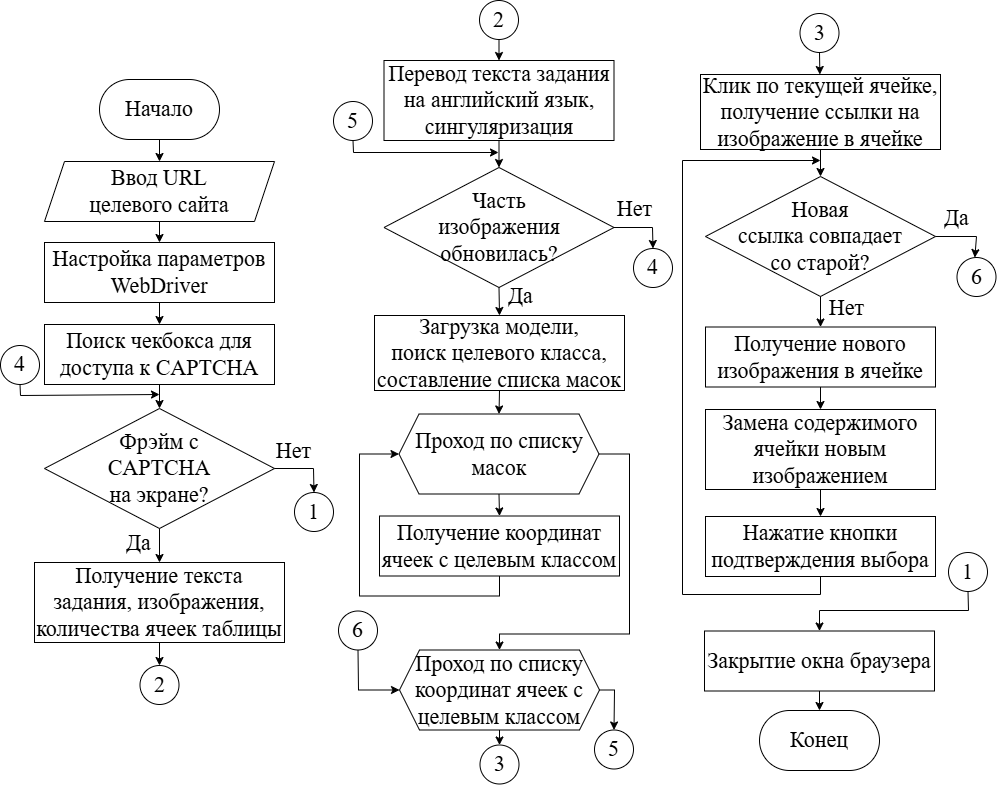
\includegraphics[width=0.6\linewidth]{imgs/solve_captcha_flow.png}
        \caption{\centering Блок-схема процесса прохождения графических CAPTCHA.}
    \end{figure}
\end{frame}

\begin{frame}{Заключение}
    \setlength{\parindent}{0.5cm}
    В результате выполненной работы были решены следующие задачи:

    \begin{enumerate}
        \item проведён обзор форматов CAPTCHA и существующих методов защиты от 
        автоматических атак;
        \item реализована система для распознавания CAPTCHA в текстовом формате 
        на основе нейросетевой модели Sequence-to-Sequence;
        \item создано решение для графических CAPTCHA с использованием модели 
        YOLO, адаптированной для распознавания объектов на изображениях;
        \item реализован подход к решению CAPTCHA в аудиоформате с использованием 
        облачного API распознавания речи;
        \item проведено тестирование всех компонентов системы в условиях, 
        приближенных к реальным, с подтверждением их корректной и стабильной 
        работы.
    \end{enumerate}
\end{frame}

\begin{frame}{Заключение}
    \setlength{\parindent}{0.5cm}
    Перспективы дальнейших исследований включают:

    \begin{enumerate}
        \item расширение набора поддерживаемых типов CAPTCHA, включая более 
        сложные динамические варианты;
        \item оптимизацию времени обработки и точности распознавания;
        \item исследование механизмов защиты CAPTCHA, устойчивых к современным 
        методам автоматического анализа.
    \end{enumerate}
\end{frame}

\end{document}
